\documentclass{book}
%\usetikzlibrary{...}% tikz package already loaded by 'tikz' option
\usepackage{template}

\begin{document}



\begin{tikzpicture}[scale=.5]
\draw[fill=gray] (0,0) rectangle (60,12);
\node at (30,6) {{\small $1$}};
    \end{tikzpicture}

\begin{tikzpicture}[scale=.5]
\draw[fill=light] (0,0) rectangle (60,12);
\draw (30,0) -- (30,12);
\node at (15,6) {{\small $\frac{1}{2}$}};
\node at (45,6) {{\small $\frac{1}{2}$}};
\end{tikzpicture}
    
   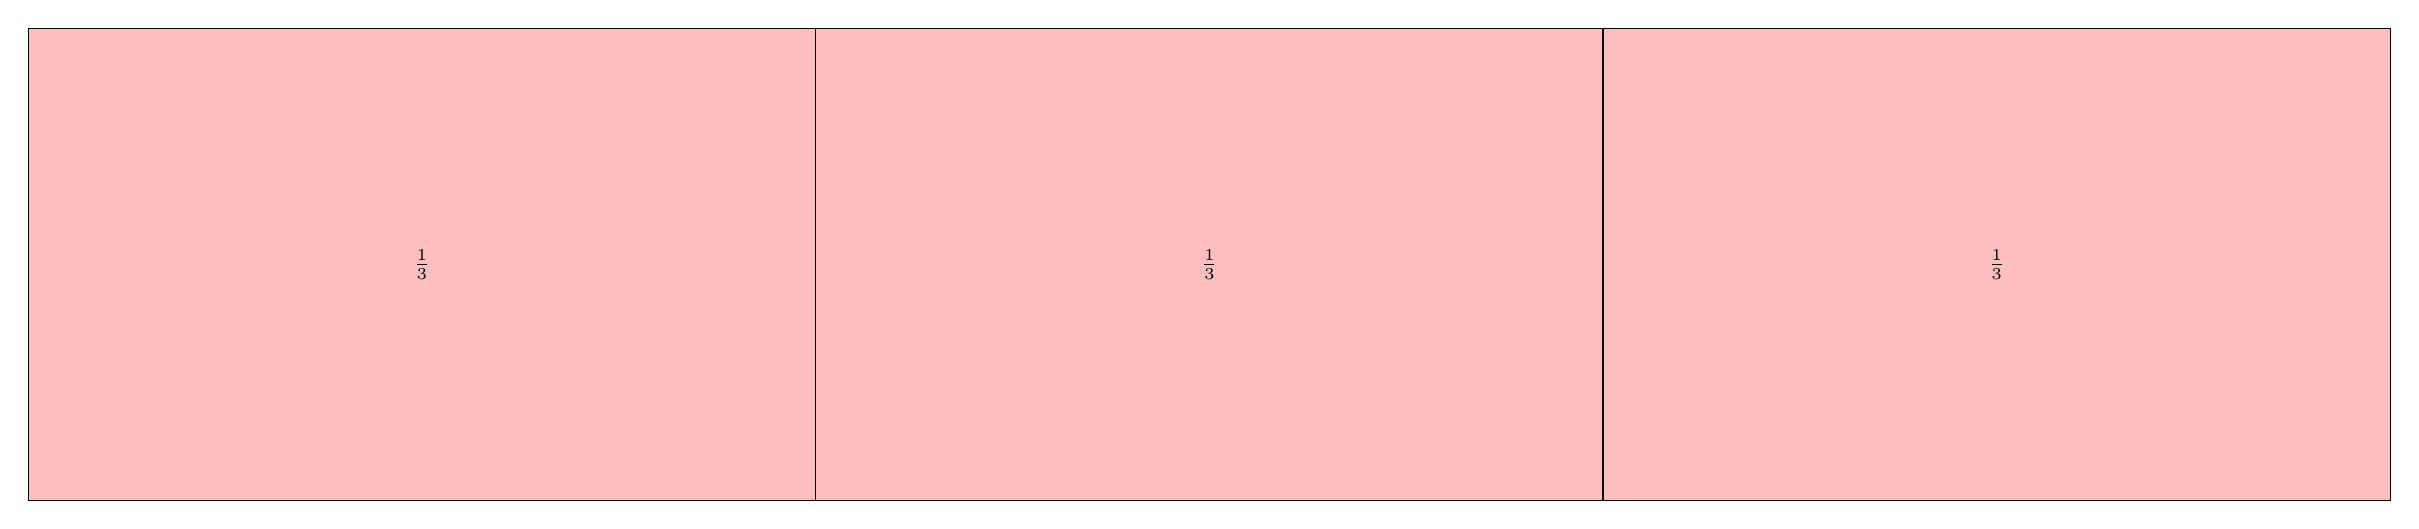
\begin{tikzpicture}[scale=.5]
\draw[fill=pink] (0,0) rectangle (60,12);
\foreach \x in {1,2} \draw (\x*60/3,0) -- (\x*60/3,12);
\foreach \x in {10,30,50} \node at (\x,6) {{\small $\frac{1}{3}$}};
    \end{tikzpicture}        
    
      \begin{tikzpicture}[scale=.5]
\draw[fill=special] (0,0) rectangle (60,12);
\foreach \x in {1,2,3} \draw (\x*60/4,0) -- (\x*60/4,12);
\foreach \x in {7.5,22.5,37.5,52.5} \node at (\x,6) {{\small $\frac{1}{4}$}};
    \end{tikzpicture}        
    
   \begin{tikzpicture}[scale=.5]
\draw[fill=attention] (0,0) rectangle (60,12);
\foreach \x in {1,...,4} \draw (\x*60/5,0) -- (\x*60/5,12);
\foreach \x in {6,18,30,42,54} \node at (\x,6) {{\small $\frac{1}{5}$}};
    \end{tikzpicture}        
    
   \begin{tikzpicture}[scale=.5]
\draw[fill=common] (0,0) rectangle (60,12);
\foreach \x in {1,...,5} \draw (\x*60/6,0) -- (\x*60/6,12);
\foreach \x in {1,3,...,12} \node at (\x*60/12,6) {{\small $\frac{1}{6}$}};
    \end{tikzpicture}        
    
    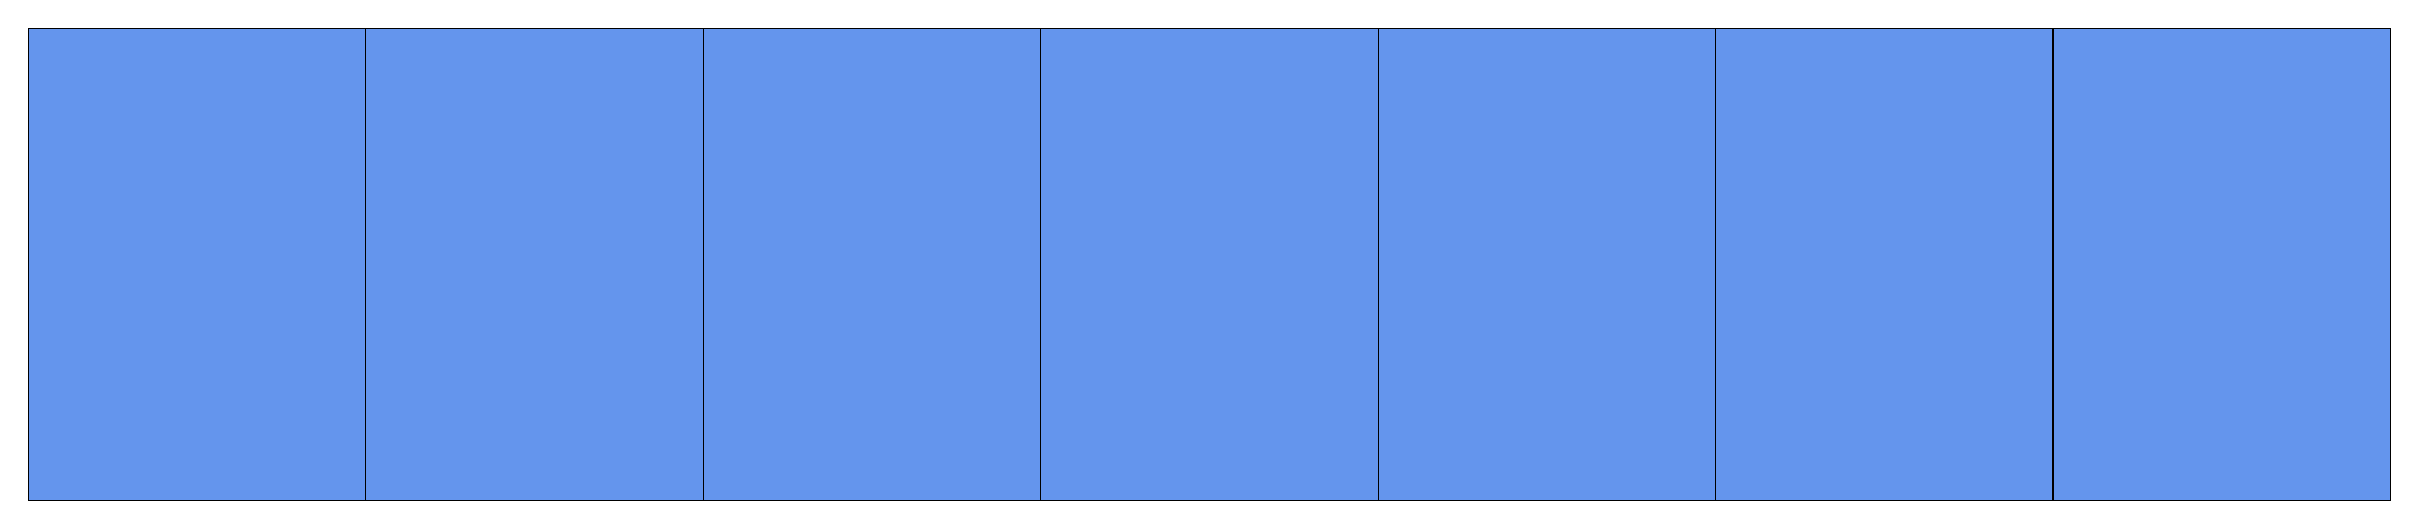
\begin{tikzpicture}[scale=.5]
\draw[fill=CornflowerBlue] (0,0) rectangle (60,12);
\foreach \x in {1,...,6} \draw (\x*60/7,0) -- (\x*60/7,12);
    \end{tikzpicture}        
    
   \begin{tikzpicture}[scale=.5]
\draw[fill=dark] (0,0) rectangle (60,12);
\foreach \x in {1,...,7} \draw (\x*60/8,0) -- (\x*60/8,12);
    \end{tikzpicture}        
    
   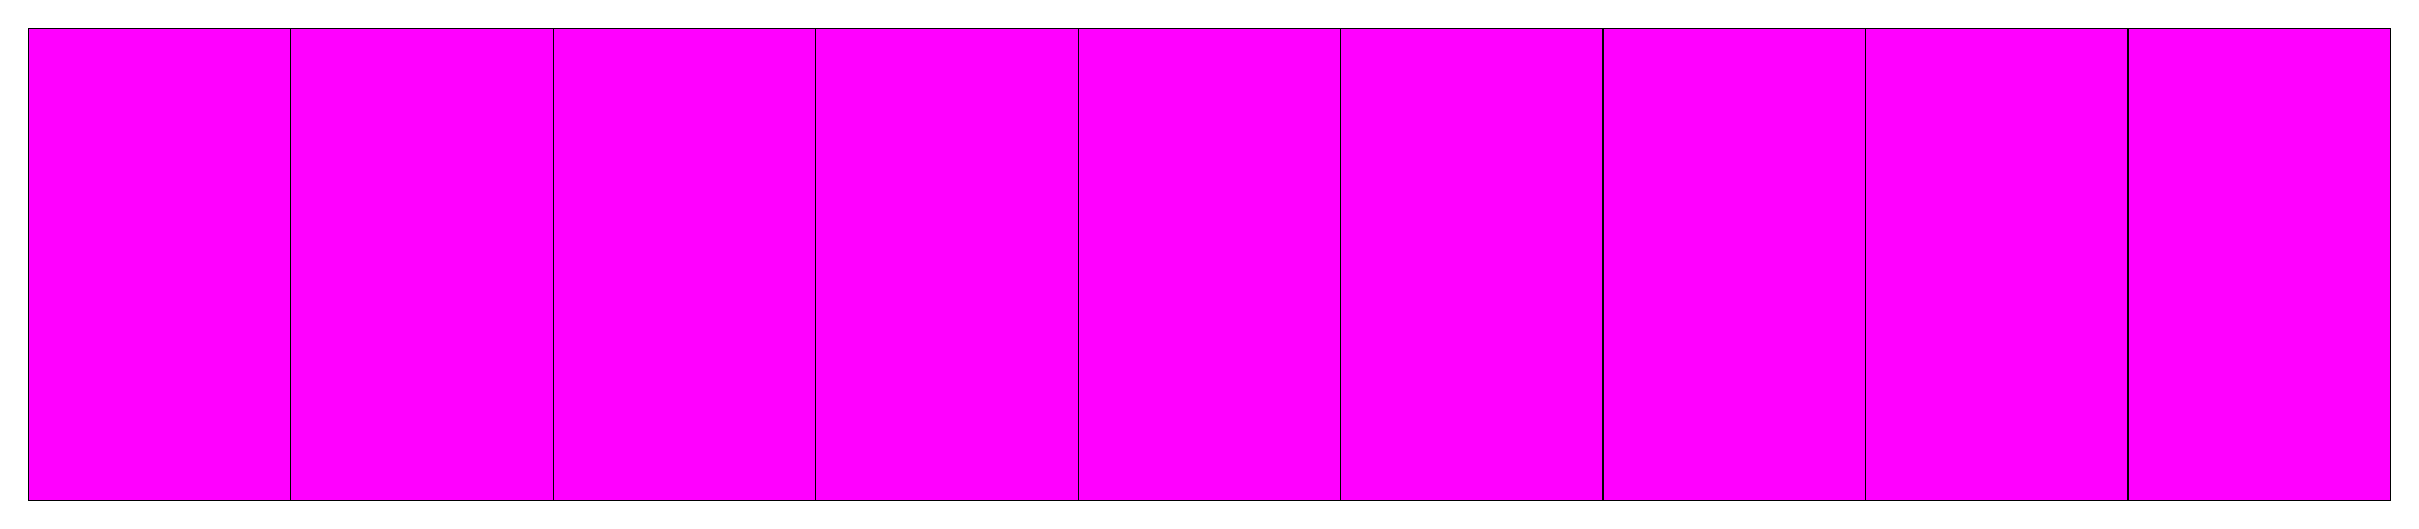
\begin{tikzpicture}[scale=.5]
\draw[fill=Fuchsia] (0,0) rectangle (60,12);'
\foreach \x in {1,...,8} \draw (\x*60/9,0) -- (\x*60/9,12);
    \end{tikzpicture}        
    
 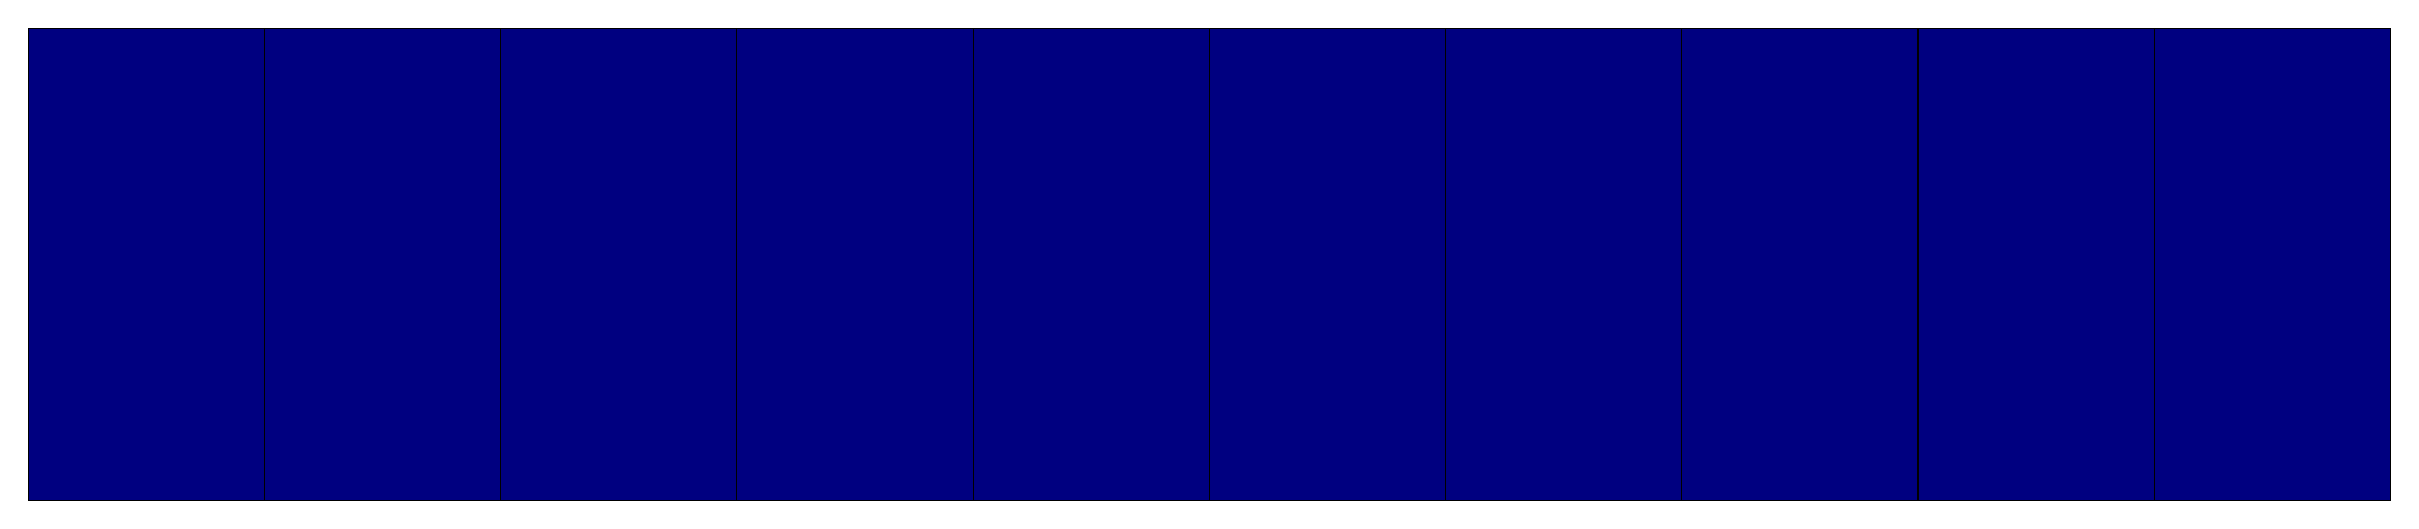
\begin{tikzpicture}[scale=.5]   
 \draw[fill=NavyBlue] (0,0) rectangle (60,12);
 \foreach \x in {1,...,9} \draw (\x*60/10,0) -- (\x*60/10,12);
     \end{tikzpicture}        
    
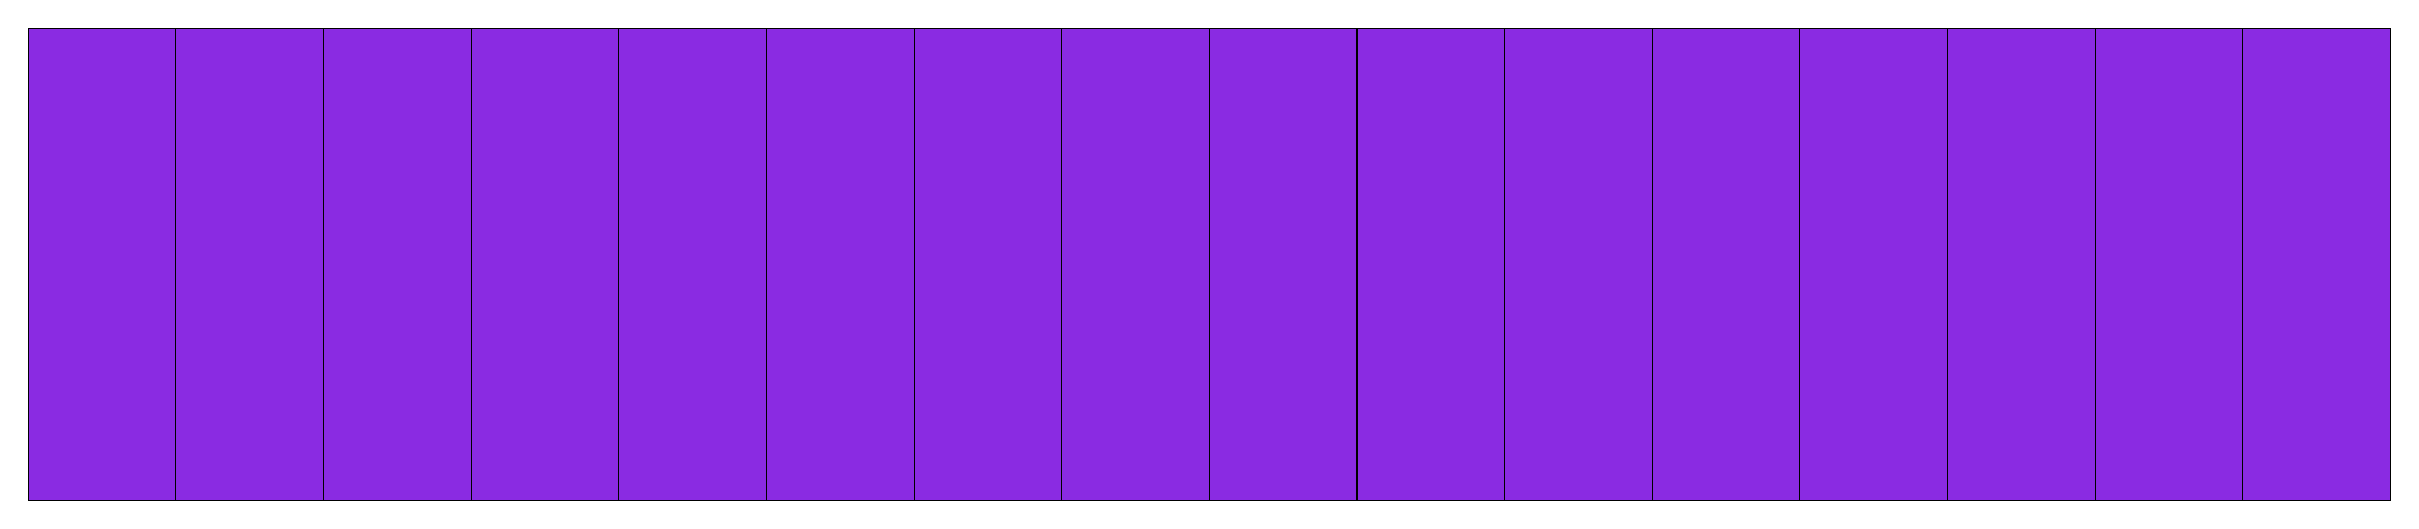
\begin{tikzpicture}[scale=.5]   
    \draw[fill=BlueViolet] (0,0) rectangle (60,12);
\foreach \x in {1,...,15} \draw (\x*60/16,0) -- (\x*60/16,12);
    \end{tikzpicture}        



\end{document}